\documentclass{article}
\usepackage{amsmath,amssymb}
\usepackage{graphicx}
\usepackage{enumerate}
\usepackage{hyperref}
\usepackage{subcaption}
\usepackage{caption}
\usepackage{xcolor}
\usepackage{float}

\pagestyle{empty} \addtolength{\textwidth}{1.0in}
\addtolength{\textheight}{0.5in}
\addtolength{\oddsidemargin}{-0.5in}
\addtolength{\evensidemargin}{-0.5in}
\newcommand{\ruleskip}{\bigskip\hrule\bigskip}
\newcommand{\nodify}[1]{{\sc #1}}
\newcommand{\points}[1]{{\textbf{[#1 points]}}}
\newcommand{\subquestionpoints}[1]{{[#1 points]}}
\newenvironment{answer}{{\bf Answer:} \sf }{}%

\newcommand{\bitem}{\begin{list}{$\bullet$}%
{\setlength{\itemsep}{0pt}\setlength{\topsep}{0pt}%
\setlength{\rightmargin}{0pt}}}
\newcommand{\eitem}{\end{list}}

\setlength{\parindent}{0pt} \setlength{\parskip}{0.5ex}
\setlength{\unitlength}{1cm}

\newcommand{\pa}[1]{[[PA: #1]]}

\renewcommand{\Re}{{\mathbb R}}
\newcommand{\E}{{\rm E}}
\begin{document}

\pagestyle{myheadings} \markboth{}{CS 294-158 Deep Unsupervised Learning, Homework 1, Spring 2020}

{\huge
\noindent Homework 1: Autoregressive Models}
\ruleskip

{\bf Deliverable}:  PDF write-up by {\bf Tuesday February 11th, 23:59pm}.  Your PDF should be generated by simply replacing the placeholder images of this LaTeX document with the appropriate solution images that will be generated automatically when solving each question. The solution images are automatically generated and saved using the accompanying IPython notebook. Your PDF is to be submitted into Gradescope. This PDF already contains a few solution images.  These images will allow you to check your own solution to ensure correctness.


\vspace{.2in}

%--------------------------------------------------------------------------------
%--------------------------------------------------------------------------------
%--------------------------------------------------------------------------------
\noindent {\bf Question 1: 1D Data}
%--------------------------------------------------------------------------------
%--------------------------------------------------------------------------------
%--------------------------------------------------------------------------------

\begin{enumerate}[(a)]

\item {\bf [10pt] Fitting a Histogram} \\\\
Final test loss for dataset 1: 2.0553 nats / dim
\begin{figure}[H]
    \centering
    \begin{subfigure}{0.45\textwidth}
        \centering
        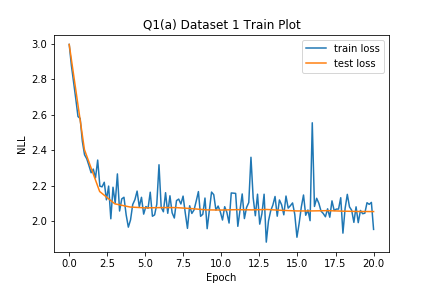
\includegraphics[width=\textwidth]{figures/q1_a_dset1_train_plot.png}
        \caption{Dataset 1: Training curve}
    \end{subfigure}
    \hspace{0.2in}
    \begin{subfigure}{0.45\textwidth}
        \centering
        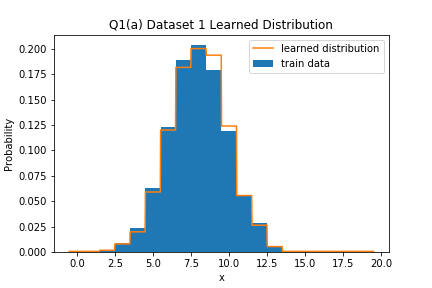
\includegraphics[width=\textwidth]{figures/q1_a_dset1_learned_dist.png}
        \caption{Dataset 1: Learned distribution}
    \end{subfigure}
\end{figure}
Final test loss for dataset 2: 0.0000  nats / dim
\begin{figure}[H]
    \centering
    \begin{subfigure}{0.45\textwidth}
        \centering
        
\includegraphics[width=\textwidth]{figures/q1_a_dset2_train_plot.png}
        \caption{Dataset 2: Training curve}
    \end{subfigure}
    \hspace{0.2in}
    \begin{subfigure}{0.45\textwidth}
        \centering
        
\includegraphics[width=\textwidth]{figures/q1_a_dset2_learned_dist.png}
        \caption{Dataset 2: Learned distribution}
    \end{subfigure}
\end{figure}

\newpage

\item {\bf [10pth] Fitting Discretized Mixture of Logistics} \\\\
Final test loss for dataset 1: 2.0586  nats / dim
\begin{figure}[H]
    \centering
    \begin{subfigure}{0.45\textwidth}
        \centering
        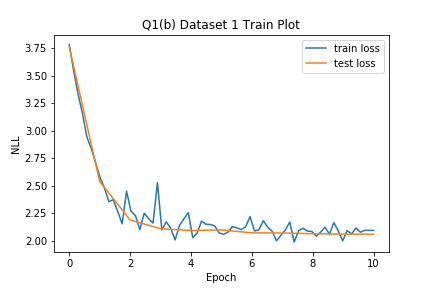
\includegraphics[width=\textwidth]{figures/q1_b_dset1_train_plot.png}
        \caption{Dataset 1: Training curve}
    \end{subfigure}
    \hspace{0.2in}
    \begin{subfigure}{0.45\textwidth}
        \centering
        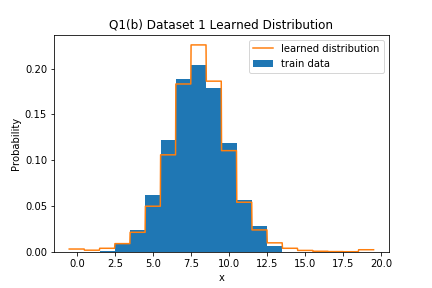
\includegraphics[width=\textwidth]{figures/q1_b_dset1_learned_dist.png}
        \caption{Dataset 1: Learned distribution}
    \end{subfigure}
\end{figure}
Final test loss for dataset 2: 0.0000  nats / dim
\begin{figure}[H]
    \centering
    \begin{subfigure}{0.45\textwidth}
        \centering
        
\includegraphics[width=\textwidth]{figures/q1_b_dset2_train_plot.png}
        \caption{Dataset 2: Training curve}
    \end{subfigure}
    \hspace{0.2in}
    \begin{subfigure}{0.45\textwidth}
        \centering
        
\includegraphics[width=\textwidth]{figures/q1_b_dset2_learned_dist.png}
        \caption{Dataset 2: Learned distribution}
    \end{subfigure}
\end{figure}
\end{enumerate}



%--------------------------------------------------------------------------------
%--------------------------------------------------------------------------------
%--------------------------------------------------------------------------------
\newpage
\noindent {\bf Question 2: MADE}
%--------------------------------------------------------------------------------
%--------------------------------------------------------------------------------
%--------------------------------------------------------------------------------

\begin{enumerate}[(a)]

\item {\bf [10pt] Fitting 2D Data} \\\\

Final test loss for dataset 1: 3.1518  nats / dim
\begin{figure}[H]
    \centering
    \begin{subfigure}{0.45\textwidth}
        \centering
        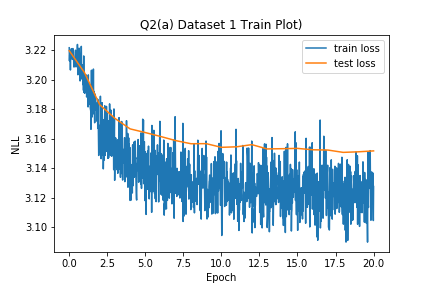
\includegraphics[width=\textwidth]{figures/q2_a_dset1_train_plot.png}
        \caption{Dataset 1: Training curve}
    \end{subfigure}
    \hspace{0.2in}
    \begin{subfigure}{0.45\textwidth}
        \centering
        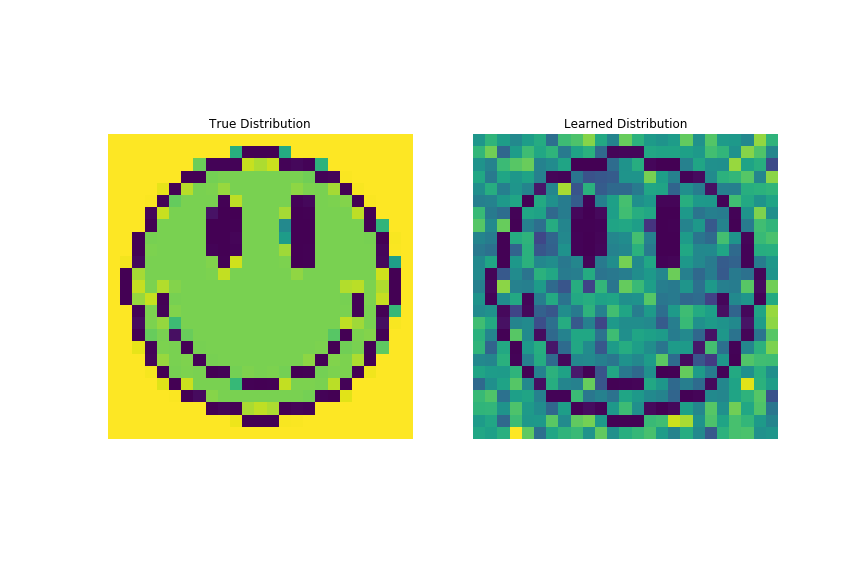
\includegraphics[width=\textwidth]{figures/q2_a_dset1_learned_dist.png}
        \caption{Dataset 1: Learned distribution}
    \end{subfigure}
\end{figure}
Final test loss for dataset 2: 0.0000  nats / dim
\begin{figure}[H]
    \centering
    \begin{subfigure}{0.45\textwidth}
        \centering
        
\includegraphics[width=\textwidth]{figures/q2_a_dset2_train_plot.png}
        \caption{Dataset 2: Training curve}
    \end{subfigure}
    \hspace{0.2in}
    \begin{subfigure}{0.45\textwidth}
        \centering
        
\includegraphics[width=\textwidth]{figures/q2_a_dset2_learned_dist.png}
        \caption{Dataset 2: Learned distribution}
    \end{subfigure}
\end{figure}

\newpage
\item {\bf [10pt] Shapes and MNIST} \\\\
Final test loss for dataset 1: 0.0623  nats / dim
\begin{figure}[H]
    \centering
    \begin{subfigure}{0.45\textwidth}
        \centering
        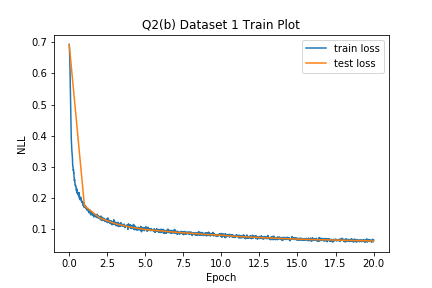
\includegraphics[width=\textwidth]{figures/q2_b_dset1_train_plot.png}
        \caption{Dataset 1: Training curve}
    \end{subfigure}
    \hspace{0.2in}
    \begin{subfigure}{0.45\textwidth}
        \centering
        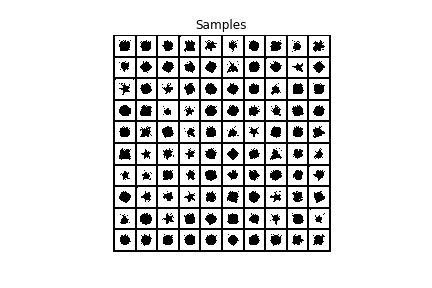
\includegraphics[width=\textwidth]{figures/q2_b_dset1_samples.png}
        \caption{Dataset 1: Samples}
    \end{subfigure}
\end{figure}
Final test loss for dataset 2: 0.0000  nats / dim
\begin{figure}[H]
    \centering
    \begin{subfigure}{0.45\textwidth}
        \centering
        
\includegraphics[width=\textwidth]{figures/q2_b_dset2_train_plot.png}
        \caption{Dataset 2: Training curve}
    \end{subfigure}
    \hspace{0.2in}
    \begin{subfigure}{0.45\textwidth}
        \centering
        
\includegraphics[width=\textwidth]{figures/q2_b_dset2_samples.png}
        \caption{Dataset 2: Samples}
    \end{subfigure}
\end{figure}

\end{enumerate}

%--------------------------------------------------------------------------------
%--------------------------------------------------------------------------------
%--------------------------------------------------------------------------------
\newpage
\noindent {\bf Question 3: PixelCNNs}
%--------------------------------------------------------------------------------
%--------------------------------------------------------------------------------
%--------------------------------------------------------------------------------

\begin{enumerate}[(a)]
\item {\bf [10pt] PixelCNNs on Binary Data} \\\\
Final test loss for dataset 1: 0.0420  nats / dim
\begin{figure}[H]
    \centering
    \begin{subfigure}{0.45\textwidth}
        \centering
        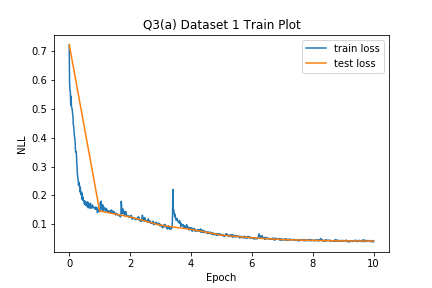
\includegraphics[width=\textwidth]{figures/q3_a_dset1_train_plot.png}
        \caption{Dataset 1: Training curve}
    \end{subfigure}
    \hspace{0.2in}
    \begin{subfigure}{0.45\textwidth}
        \centering
        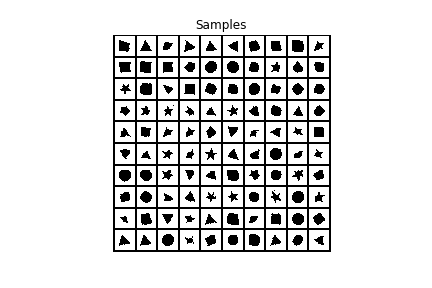
\includegraphics[width=\textwidth]{figures/q3_a_dset1_samples.png}
        \caption{Dataset 1: Samples}
    \end{subfigure}
\end{figure}
Final test loss for dataset 2: 0.0000  nats / dim
\begin{figure}[H]
    \centering
    \begin{subfigure}{0.45\textwidth}
        \centering
        
\includegraphics[width=\textwidth]{figures/q3_a_dset2_train_plot.png}
        \caption{Dataset 2: Training curve}
    \end{subfigure}
    \hspace{0.2in}
    \begin{subfigure}{0.45\textwidth}
        \centering
        
\includegraphics[width=\textwidth]{figures/q3_a_dset2_samples.png}
        \caption{Dataset 2: Samples}
    \end{subfigure}
\end{figure}

\newpage

\item {\bf [10pt] Independent Color Channels} \\\\
Final test loss for dataset 1: 0.0444  nats / dim
\begin{figure}[H]
    \centering
    \begin{subfigure}{0.45\textwidth}
        \centering
        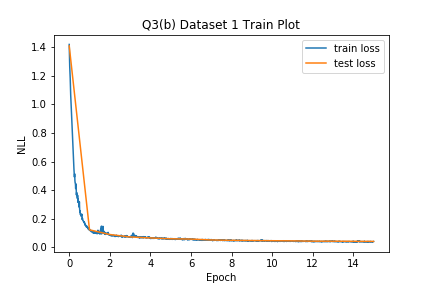
\includegraphics[width=\textwidth]{figures/q3_b_dset1_train_plot.png}
        \caption{Dataset 1: Training curve}
    \end{subfigure}
    \hspace{0.2in}
    \begin{subfigure}{0.45\textwidth}
        \centering
        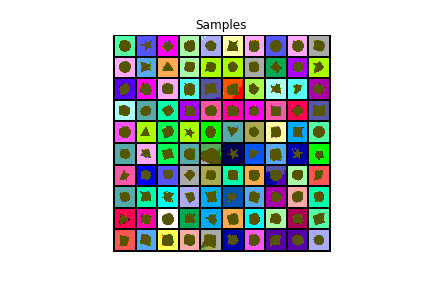
\includegraphics[width=\textwidth]{figures/q3_b_dset1_samples.png}
        \caption{Dataset 1: Samples}
    \end{subfigure}
\end{figure}
Final test loss for dataset 2: 0.0000  nats / dim
\begin{figure}[H]
    \centering
    \begin{subfigure}{0.45\textwidth}
        \centering
        
\includegraphics[width=\textwidth]{figures/q3_b_dset2_train_plot.png}
        \caption{Dataset 2: Training curve}
    \end{subfigure}
    \hspace{0.2in}
    \begin{subfigure}{0.45\textwidth}
        \centering
        
\includegraphics[width=\textwidth]{figures/q3_b_dset2_samples.png}
        \caption{Dataset 2: Samples}
    \end{subfigure}
\end{figure}

\newpage

\item {\bf [10pt] Dependent Color Channels} \\\\
Final test loss for dataset 1: 0.0236  nats / dim
\begin{figure}[H]
    \centering
    \begin{subfigure}{0.45\textwidth}
        \centering
        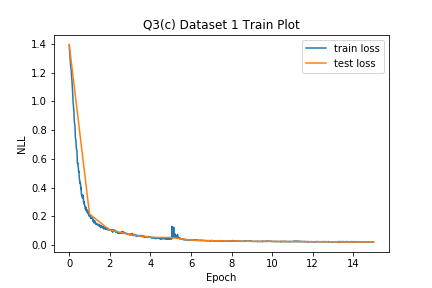
\includegraphics[width=\textwidth]{figures/q3_c_dset1_train_plot.png}
        \caption{Dataset 1: Training curve}
    \end{subfigure}
    \hspace{0.2in}
    \begin{subfigure}{0.45\textwidth}
        \centering
        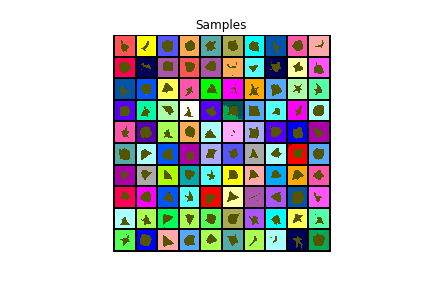
\includegraphics[width=\textwidth]{figures/q3_c_dset1_samples.png}
        \caption{Dataset 1: Samples}
    \end{subfigure}
\end{figure}
Final test loss for dataset 2: 0.0000  nats / dim
\begin{figure}[H]
    \centering
    \begin{subfigure}{0.45\textwidth}
        \centering
        
\includegraphics[width=\textwidth]{figures/q3_c_dset2_train_plot.png}
        \caption{Dataset 2: Training curve}
    \end{subfigure}
    \hspace{0.2in}
    \begin{subfigure}{0.45\textwidth}
        \centering
        
\includegraphics[width=\textwidth]{figures/q3_c_dset2_samples.png}
        \caption{Dataset 2: Samples}
    \end{subfigure}
\end{figure}

\newpage

\item {\bf [10pt] Conditional PixelCNNs} \\\\
Final test loss for dataset 1: 0.0368  nats / dim
\begin{figure}[H]
    \centering
    \begin{subfigure}{0.45\textwidth}
        \centering
        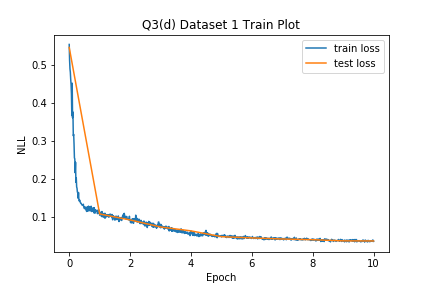
\includegraphics[width=\textwidth]{figures/q3_d_dset1_train_plot.png}
        \caption{Dataset 1: Training curve}
    \end{subfigure}
    \hspace{0.2in}
    \begin{subfigure}{0.45\textwidth}
        \centering
        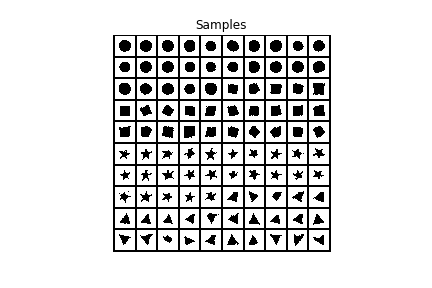
\includegraphics[width=\textwidth]{figures/q3_d_dset1_samples.png}
        \caption{Dataset 1: Samples}
    \end{subfigure}
\end{figure}
Final test loss for dataset 2: 0.0000  nats / dim
\begin{figure}[H]
    \centering
    \begin{subfigure}{0.45\textwidth}
        \centering
        
\includegraphics[width=\textwidth]{figures/q3_d_dset2_train_plot.png}
        \caption{Dataset 2: Training curve}
    \end{subfigure}
    \hspace{0.2in}
    \begin{subfigure}{0.45\textwidth}
        \centering
        
\includegraphics[width=\textwidth]{figures/q3_d_dset2_samples.png}
        \caption{Dataset 2: Samples}
    \end{subfigure}
\end{figure}

\end{enumerate}

\newpage
\noindent {\bf Bonus Questions (Optional)}
\item {\bf [10pt] Gated PixelCNN} \\\\
Final test loss: 0.0000  nats / dim
\begin{figure}[H]
    \centering
    \begin{subfigure}{0.45\textwidth}
        \centering
        
\includegraphics[width=\textwidth]{figures/q4_a_train_plot.png}
        \caption{Training curve}
    \end{subfigure}
    \hspace{0.2in}
    \begin{subfigure}{0.45\textwidth}
        \centering
        
\includegraphics[width=\textwidth]{figures/q4_a_samples.png}
        \caption{Samples}
    \end{subfigure}
\end{figure}

\newpage

\item {\bf [10pt] PixelCNN with Mixture of Logistics} \\\\
Final test loss: 0.0000  nats / dim
\begin{figure}[H]
    \centering
    \begin{subfigure}{0.45\textwidth}
        \centering
        
\includegraphics[width=\textwidth]{figures/q4_b_train_plot.png}
        \caption{Training curve}
    \end{subfigure}
    \hspace{0.2in}
    \begin{subfigure}{0.45\textwidth}
        \centering
        
\includegraphics[width=\textwidth]{figures/q4_b_samples.png}
        \caption{Samples}
    \end{subfigure}
\end{figure}
\newpage
\item {\bf [10pt] Conditioning on Auxiliary Variables} \\\\
Final test loss: 0.0000  nats / dim
\begin{figure}[H]
    \centering
    \begin{subfigure}{0.45\textwidth}
        \centering
        
\includegraphics[width=\textwidth]{figures/q4_c_train_plot.png}
        \caption{Training curve}
    \end{subfigure}
    \hspace{0.2in}
    \begin{subfigure}{0.45\textwidth}
        \centering
        
\includegraphics[width=\textwidth]{figures/q4_c_samples.png}
        \caption{Samples}
    \end{subfigure}
\end{figure}
\newpage
\item {\bf [10pt] Faster Sampling} \\\\
Final test loss: 0.0000  nats / dim
\begin{figure}[H]
    \centering
    \begin{subfigure}{0.45\textwidth}
        \centering
        
\includegraphics[width=\textwidth]{figures/q4_d_train_plot.png}
        \caption{Training curve}
    \end{subfigure}
    \hspace{0.2in}
    \begin{subfigure}{0.45\textwidth}
        \centering
        
\includegraphics[width=\textwidth]{figures/q4_d_samples.png}
        \caption{Samples}
    \end{subfigure}
\end{figure}

\end{document}
